\documentclass{article}
\usepackage[UTF8]{ctex}
\usepackage{amsmath}
\usepackage{fancyhdr}
\usepackage{geometry}
\usepackage{pgf-pie}
\usepackage{sectsty}
\usepackage{xcolor}

\geometry{left=3cm, right=3cm, top=3cm, bottom=3cm}

\title{第二次作业}
\author{Koorye}
\date{2024年3月20日}

\pagestyle{fancy}
\fancyhead[L]{移动计算技术——第二次作业}
\fancyhead[R]{Koorye}
\fancyfoot[R]{基于\LaTeX 排版制作}

\begin{document}
\maketitle
\thispagestyle{fancy}

\section{能否设计一种非代理的移动IP路由数据投递方法?}

我认为设计一种非代理的移动IP路由数据投递方法是\textbf{可行}的。

在解释原因之前,我们先来了解一下代理的移动IP路由数据投递方法。移动IP技术是一种基于IP的移动性支持技术,它通过代理的方式实现了移动设备跨越到其他网段时,保持固定IP的连接。其实现方式如下:

\begin{enumerate}
    \item \textbf{转交地址注册}。移动设备在移动到新的网段时,会向当前网段的代理服务器\textit{(外部代理)}注册一个转交地址。
    \item \textbf{转交地址登记}。外部代理会与移动设备之前所在网段的代理服务器\textit{(本地代理)}建立连接,告知其转交地址。
    \item \textbf{数据发送}。移动设备发送数据时,直接将源地址设置成之前所在网段的地址\textit{(永久地址)}。
    \item \textbf{数据接收}。\textit{本地代理}接收到数据后,根据\textit{转交地址},将数据转发给\textit{外部代理}。
\end{enumerate}

设计一种非代理的移动IP路由数据投递方法是可行的,具体来说,可以通过以下方式实现:

\begin{enumerate}
    \item \textbf{关联地址获取}。移动设备在移动到新的网段时,可以通过路由器获取一个\textit{关联地址}。
    \item \textbf{关联地址绑定}。移动设备将\textit{关联地址}与之前所在网段的地址\textit{(永久地址)}发送给正在连接的目标。目标路由器将\textit{关联地址}与\textit{永久地址}绑定。
    \item \textbf{数据发送}。移动设备发送数据时,直接将源地址设置成\textit{永久地址}。
    \item \textbf{数据接收}。目标路由器接收到数据后,通过查询\textit{永久地址}对应的\textit{关联地址},将数据转发给移动设备。
\end{enumerate}

图\ref{fig:ip}给出了代理和非代理的移动IP路由数据投递方法的对比。从图中可以看出,该方法的优势在于不需要代理服务器,减少了网络负担,提高了数据传输效率。但是,该方法也存在一些问题,比如需要目标路由器支持,且需要在网络中增加一些额外的信息,增加了网络的复杂度。由于目前IPV4技术的限制,大多数路由器并没有内部数据结构的支持,这种方法的实际应用还存在很大困难,需要网络厂商、运营商对协议进行统一的支持和改进。

\begin{figure}[htbp]
    \centering
    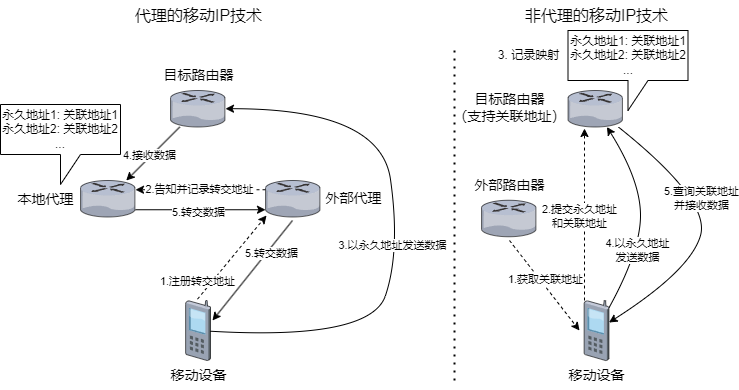
\includegraphics[width=\textwidth]{示意.drawio.png}
    \caption{代理和非代理的移动IP路由数据投递方法}
    \label{fig:ip}
\end{figure}

\end{document}